% !TEX encoding = UTF-8 Unicode

\documentclass[aspectratio=169]{beamer}
\usepackage[utf8]{inputenc}

%% GRAPHICS

\usepackage{graphicx}
\graphicspath{{images/},{figures/}}
\usepackage{tikz}
\usetikzlibrary{graphs}

%% COLORS
\definecolor{UWRed}{HTML}{C5050C}
\definecolor{TintedBG}{HTML}{EEEEFF}
\definecolor{DarkGreen}{HTML}{10A010}
\definecolor{LightGreen}{HTML}{A0FFA0}

%% SLIDE COLOR SETTINGS
\setbeamercolor{structure}{fg=UWRed}
\setbeamercolor{title page}{fg=white}
\setbeamercolor{title}{fg=white}

%% RM NAV SYMBOLS
\setbeamertemplate{navigation symbols}{}

%% FONTS
\setbeamerfont{title}{size=\huge\bfseries}

%% LOGO on slides
\logo{\begin{tikzpicture}[overlay]
	\node[anchor=north east,inner sep=0] at (0,86mm) {
\includegraphics[height=10mm]{SMPH_color-flush.pdf}};
	\end{tikzpicture}}

%% CONTENT BEGINS

\title{Database Concepts}
\subtitle{BMI 773: Clinical Research Informatics}
\author{Yuriy Sverchkov}
\institute{University of Wisconsin--Madison}
\date{February 10, 2020}

\begin{document}
	
	{
		\setbeamertemplate{background canvas}{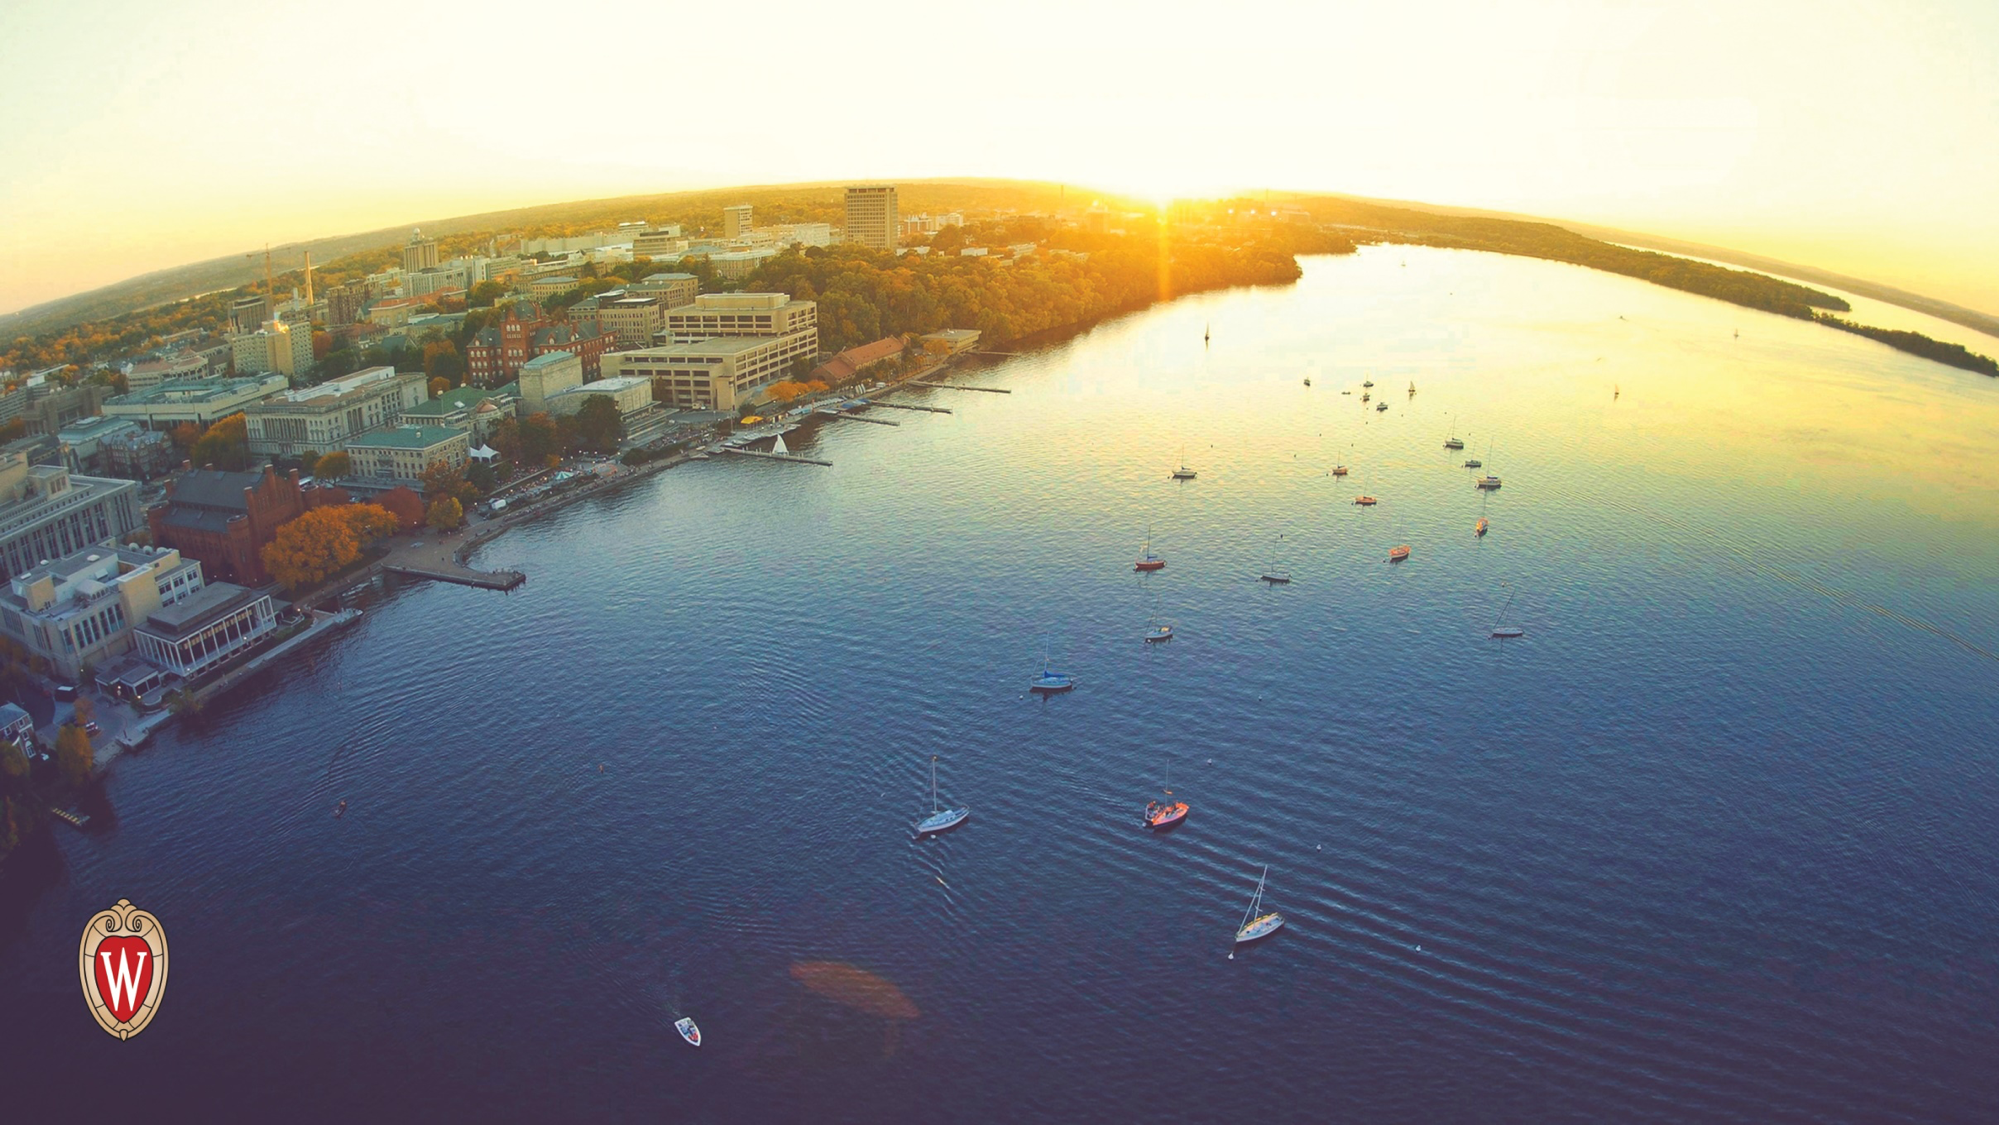
\includegraphics[width=\paperwidth]{UW-lake.png}}
		\begin{frame}[plain]
			\vskip4cm
			\titlepage
		\end{frame}
	}

	\begin{frame}{Database Concepts}
		\begin{itemize}
			\item Transactional databases vs data warehouses
			\item The relational model
			\begin{itemize}
				\item Tables, records, and columns
				\item Schemas
				\item Normal forms
				\item Keys
			\end{itemize}
			\item How to design and execute SQL queries
		\end{itemize}
	\end{frame}

	\begin{frame}{Transactional databases vs data warehouses}
		\centering
		
		%\begin{tikzpicture}
		%	\graph [branch right sep, grid placement, nodes={draw, align=left, text width=0.3\linewidth}] { [n=15, wrap after=3]
		%		/, /{\bf Transactional database}, /{\bf Data warehouse},
		%		Purpose, /{Maintain up-to-date record of events}, Collect and aggregate historical data,
		%		Update frequency, /{In real-time}, /{Periodically (a few times per day or less)},
		%		Optimized for, /{Fast updates, fast look-up of individual patients}, /{Analytics, searches of collections},
		%%	};
		%\end{tikzpicture}
		
		\begin{tabular}{lp{0.3\linewidth}p{0.3\linewidth}}
			& \textbf{Transactional database} & \textbf{Data warehouse} \\
			Purpose & Support day-to-day operations & Collect and aggregate data for analysis \\
			Update frequency & In real-time & Periodically (a few times per day or less) \\
			Optimized for & Fast updates, fast look-up of individual patients & Analytics, searches of collections \\
			Epic e.g. & Chronicles & Clarity and Caboodle
		\end{tabular}
		
	\end{frame}

	% Not all DBs are relational:
	% e.g. Chronicles uses InterSystems Caché, which is a hierarchical database
	% It's actually very popular choice for the transactional system

	\begin{frame}{}
		\centering
		\begin{tikzpicture}[
			whitenode/.style={fill=white, draw=none},
			bluenode/.style={fill=blue!20, draw=blue!80},
			greennode/.style={fill=LightGreen, draw=DarkGreen}
		]
			\matrix (table) [
			ampersand replacement=\&,
			row sep=0.1cm, column sep=0.1cm,
			nodes={minimum width=2.5cm, minimum height=0.8cm, draw=black!80, very thick, fill=black!20, font=\ttfamily}
			] {
				\node[whitenode] {first\_name}; \& \node[whitenode] (attr) {\color<2>{blue!80}{last\_name}}; \&  \node[whitenode] {gender}; \& \node[whitenode] {birth\_date};\\
				\node {Lauren}; \& \alt<2>{\node[bluenode] }{\node } {Johnson}; \& \node {F}; \& \node {1982-03-12}; \\
				\alt<3>{\node[greennode] (record)}{\node (record)} {Peter}; \& \alt<2>{\node[bluenode]}{\alt<3>{\node[greennode]}{\node}} {Jurasik}; \& \alt<3>{\node[greennode]}{\node} {M}; \&  \alt<3>{\node[greennode]}{\node} {1950-04-25};  \\
				\node {Richard}; \& \alt<2>{\node[bluenode]}{\node} {Biggs}; \& \node {M}; \& \node {1960-03-18}; \\
				\node {Lauren}; \& \alt<2>{\node[bluenode]}{\node} {Johnson}; \& \node {F}; \& \node {1974-06-01}; \\
			};
		
			\only<1->{
				\node[anchor=south east, color=purple!80, font=\bfseries, align=center] at (table.north west) {Table\\ Relation\\ Relvar}; }
			\only<2->{
				\node[anchor=south, color=blue!80, font=\bfseries, align=center] at (attr.north) {Column\\Attribute\\Field};
			}
			\only<3->{
				\node[anchor=east, color=DarkGreen, font=\bfseries, align=center] at (record.west) {Row\\Tuple\\Record};
			}
		\end{tikzpicture}
	\end{frame}

	% Do a thing on primary key/surrogate key/natural key?

	\begin{frame}{Why have more than one table?}
	
	{\tiny
		\begin{tabular}{lllllll}
			\bf First Name & \bf Last Name & \bf Birth date \only<2->{& \bf Drug & \bf Prescription date} \only<3>{& \bf Drug 2 & \bf Prescription date 2} \\ \hline
			Lauren & Johnson & 1982-03-12 \only<2->{& Acetaminophen & 2010-01-06} \only<3>{& --- & ---} \\
			Alice & Smith & 1979-12-04 \only<2->{& Amoxicillin & 1998-01-29 } \only<3>{& Lisinopril & 2019-05-26 } \\
			\only<4->{Alice & Smith & 1979-12-04 & Lisinopril & 2019-05-26 \\}
			James & White & 1964-09-01 \only<2->{& Albuterol & 1990-12-15 } \only<3>{& --- & ---} \\
		\end{tabular}
	}
	\vfill
		\begin{itemize}
			\item Consider a database of patients \only<2->{and their prescriptions}
			\item<2-> How can we track multiple prescriptions for a patient?
				\begin{itemize}
					\item<3-> Add columns?
					\item<4-> One row per prescription?
				\end{itemize}
		\end{itemize}
	\end{frame}

	\begin{frame}
		
		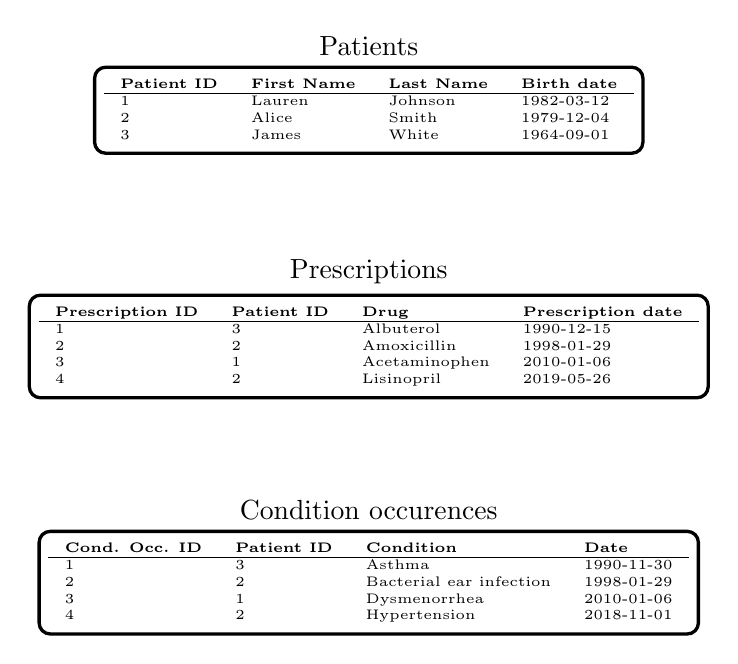
\begin{tikzpicture}
			\node[label=Patients, draw, very thick, rounded corners] (patient) at (0,0) {\tiny
				\begin{tabular}{llll}
				\bf Patient ID & \bf First Name & \bf Last Name & \bf Birth date \\ \hline
				1 &	Lauren & Johnson & 1982-03-12 \\
				2 & Alice & Smith & 1979-12-04 \\
				3 & James & White & 1964-09-01 \\
				\end{tabular}
			};
			\node[label=Prescriptions, draw, very thick, rounded corners] (drug) at (0,-3cm) {\tiny
				\begin{tabular}{llll}
				\bf Prescription ID & \bf Patient ID & \bf Drug & \bf Prescription date \\ \hline
				1 & 3 & Albuterol & 1990-12-15 \\
				2 & 2 & Amoxicillin & 1998-01-29 \\
				3 & 1 & Acetaminophen & 2010-01-06 \\
				4 & 2 & Lisinopril & 2019-05-26 \\
				\end{tabular}
			};
			\uncover<2->{
			\node[label=Condition occurences, draw, very thick, rounded corners] at (0, -6cm) {\tiny
				\begin{tabular}{llll}
				\bf Cond. Occ. ID & \bf Patient ID & \bf Condition & \bf Date \\ \hline
				1 & 3 & Asthma & 1990-11-30 \\
				2 & 2 & Bacterial ear infection & 1998-01-29 \\
				3 & 1 & Dysmenorrhea & 2010-01-06 \\
				4 & 2 & Hypertension & 2018-11-01
				\end{tabular}
			};}
		\end{tikzpicture}
	
		%TODO: Visit + arrows
	\end{frame}


	% Something about multidimensionality?

	\begin{frame}
		
		\begin{columns}
			\column{0.5\linewidth}
				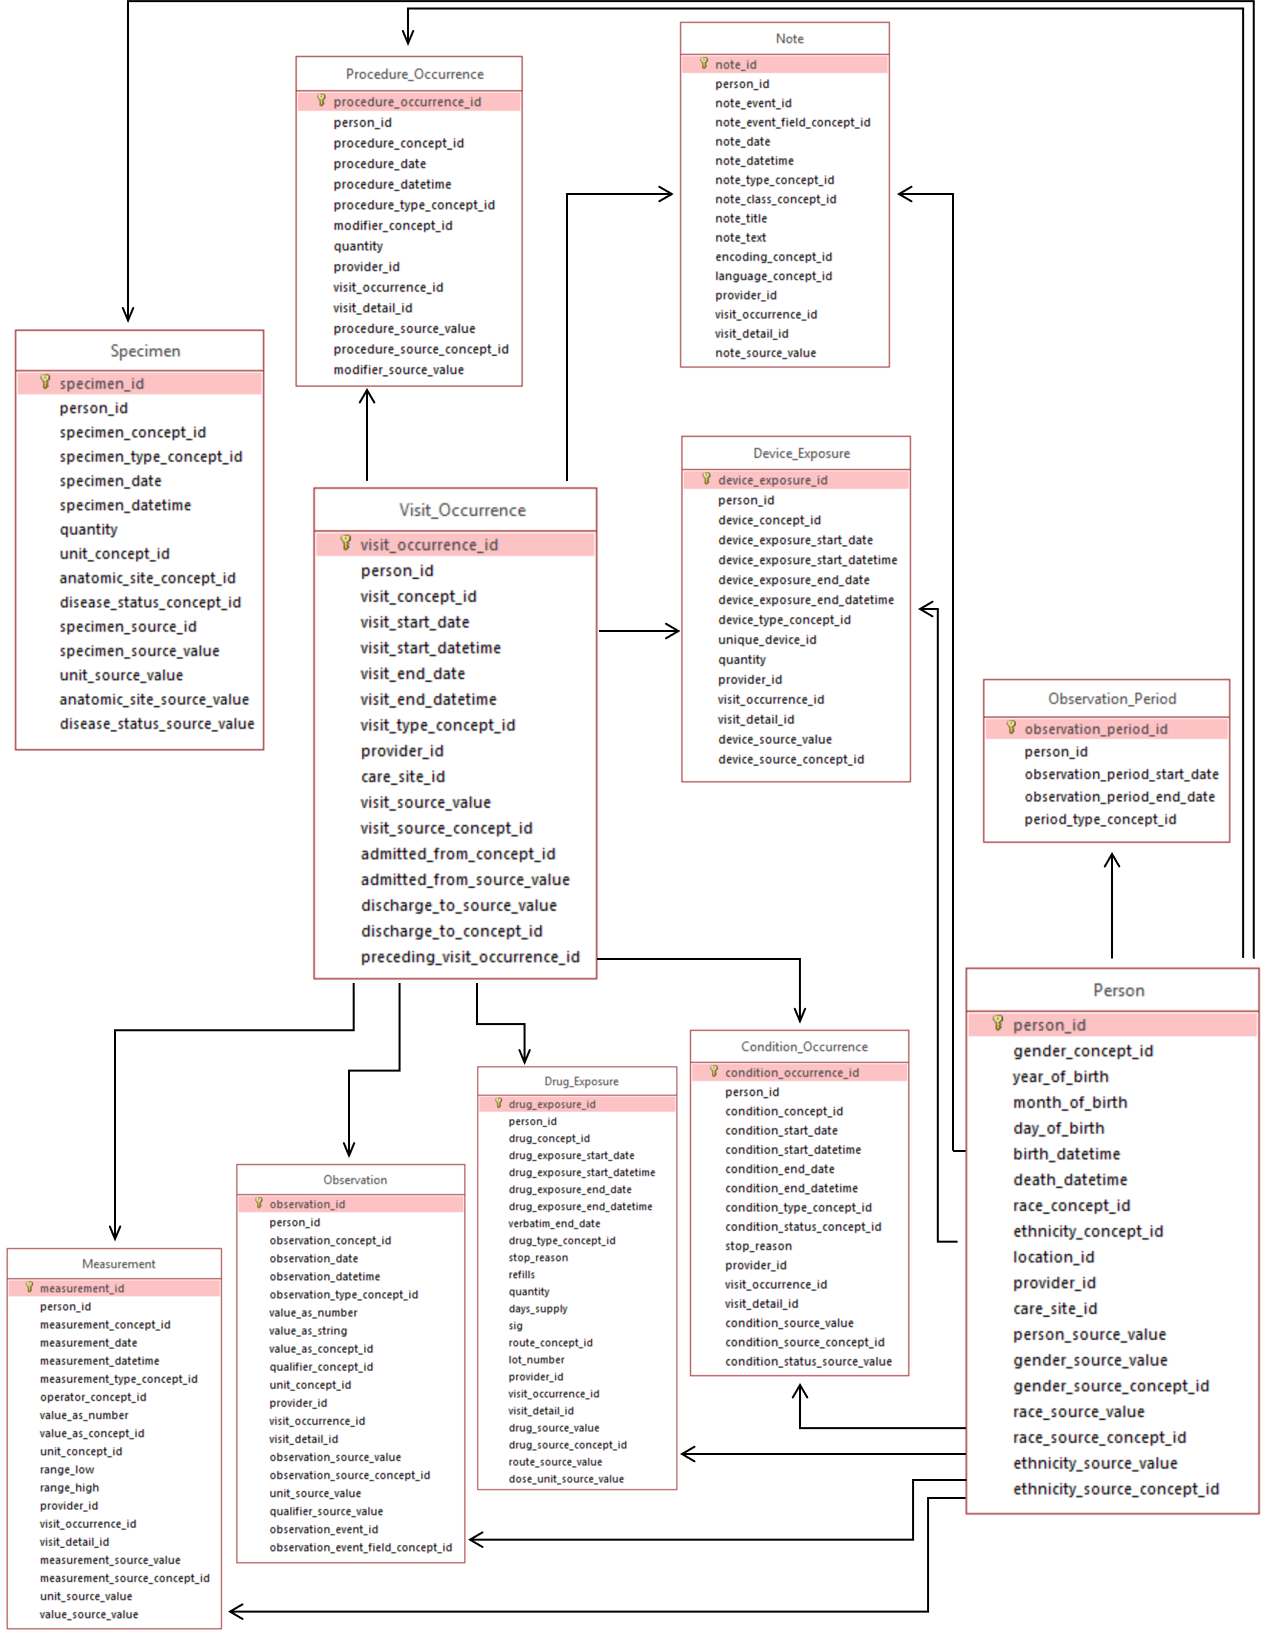
\includegraphics[height=8.5cm]{ohdsi_clinical_schema}
			\column{0.5\linewidth}
			\small
				\begin{itemize}
					\item A \textbf{database schema} describes the structure of a relational database
					\begin{itemize}
						\item Tables
						\item Columns
						\item Primary and foreign keys
					\end{itemize}
					\item There are a few formal standards for graphically representing a schema graphically: object-role models (ORM) and multiple standards for Entity-relationship (ER) diagrams.
					\item Example: OHDSI Common Data Model Clinical Tables Schema
				\end{itemize}
		\end{columns}		
	\end{frame}

	\begin{frame}{Structured Query Language (SQL)}
		
		\begin{itemize}[<+->]
			\item A language for managing data in relational database management systems (RDBMS)
			\item There are differences in dialects and implementation between different RDBMS providers
			\item SQL has functionality for data query, data manipulation (adding/deleting/modifying records), data definition (defining a schema) and data access control (managing user access to the database).
			\item We will focus on data query
		\end{itemize}
	\end{frame}

	\begin{frame}{SQL SELECT}
	\end{frame}

\end{document}